\section{Non-Preemptive Protocol}

\subsection{Definition}

This protocol is a simple protocol and named non preemptive because it avoid any interruption on running task $\tau_{j}$ that accessing a resource $ R_{k} $that guarded by , $ S_{k} $. To reduce total blocking time experienced by the task $\tau_{i}$ that have highest priority, this protocol just increase the priority of the task $\tau_{j}$ that currently accessing the resource $\tau_{j}$, so that the task will not be interrupted and can be done much faster.Without this protocol, the task that highest priority $\tau_{i}$ will interrupt the task $\tau_{j}$ that currently accessing the resource $ R_{k} $ even though the task cannot access the resource because it already guarded by $ S_{k} $. The scheduler then switch back to the task before to finish its process, this switch context process could cause longer blocking time experienced by the highest priority task. After the task$\tau_{j}$ finish accessing the resources, its priority will be back to its nominal priority $ P_{j} $.These situations can be compared through figure \ref{fig:An_example_of_priority_inversion} and \ref{fig:Example_of_NPP_preventing_priority_inversion} . So, the priority of the task $\tau_{i}$that currently accessing the resource is 

\begin{center}
$p_{i}(R_{k})=\underset{h}{\mathrm{max}} \{P_{h}\}  $

\end{center}

\begin{figure}[h]
    \centering
    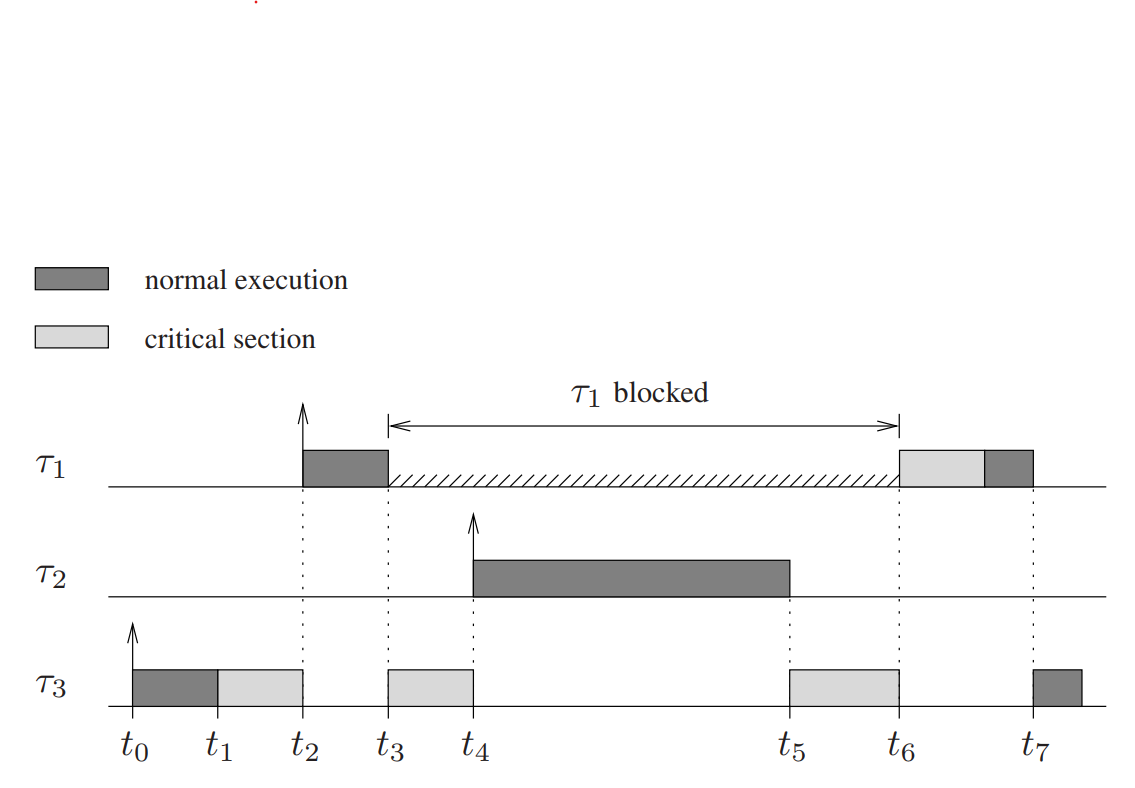
\includegraphics[width=0.5\textwidth]{An_example_of_priority_inversion}
    \caption{An example of priority inversion.. \cite{b5}}
    \label{fig:An_example_of_priority_inversion}
\end{figure}

\begin{figure}[h]
    \centering
    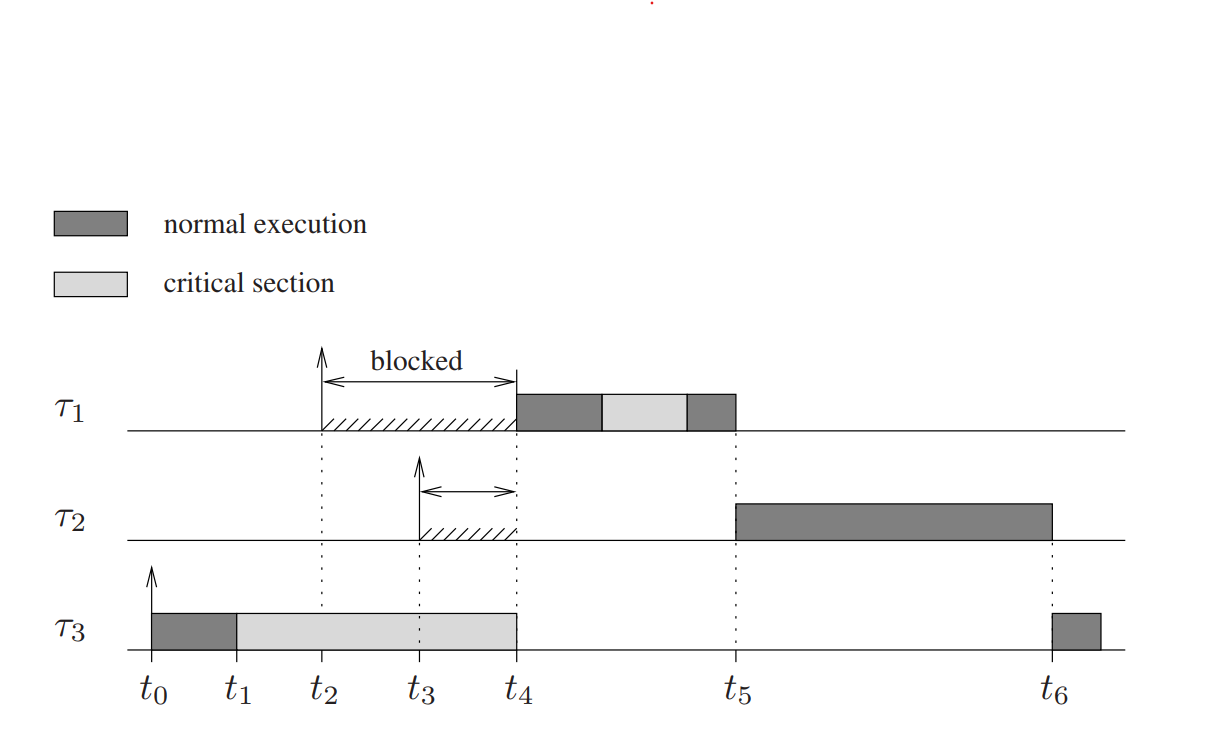
\includegraphics[width=0.5\textwidth]{Example_of_NPP_preventing_priority_inversion}
    \caption{Example of NPP preventing priority inversion. \cite{b5}}
    \label{fig:Example_of_NPP_preventing_priority_inversion}
\end{figure}


\subsection{Blocking time computation}

	The total of critical section of lower priority task $\tau_{j}$ blocking higher priority task $\tau_{i}$ is

\begin{center}
$ \gamma_{i}=\{Z_{j,k} | P_{j}<P_{i}, k=1,...,m \} $ \cite{b5}
\end{center}

Hence the total duration highest priority task is blocked is

\begin{center}

$B_{i}(R_{k})=\underset{j,k}{\mathrm{max}} \{ \delta_{j,k}-1 | Z_{j,k} \in \gamma_{i}\}  $ \cite{b5}
\end{center}

\subsection{Implementation Strategies}

As state by \cite{b6} - All commercial RTOSs have a means for beginning and ending a critical section. Invoking this Scheduler 
operation prevents all task switching from occurring during the critical section. If we write our own RTOS, the most common way to do this is to set the Disable Interrupts bit on our processor's flags register. The precise details of this vary, naturally, depending on the specific processor.

\subsection{Sample Model}

The following example model is totally taken from \cite{b6}.

An example of the use of this pattern is shown in Figure \ref{fig:npp_model}. This example contains three tasks: Device Test (highest priority), Motor Control (medium priority), and Data Processing (lowest priority). Device Test and Data Processing share a resource called Sensor, whereas Motor Control has its own resource called Motor. 

The scenario starts off with the lowest-priority task, Data Processing, accessing the resource that starts up a critical section. During this critical section both the Motor Control task and the Device Test task become ready to run but cannot because task switching is disabled. When the call to the resource is almost done, the Sensor.gimme() operation makes a call to the scheduler to end the critical section. The scenario shows three critical sections, one for each of the running tasks. Finally, at the end, the lowest-priority task is allowed to complete its work and then returns to its Idle state.

\begin{figure}[h]
    \centering
    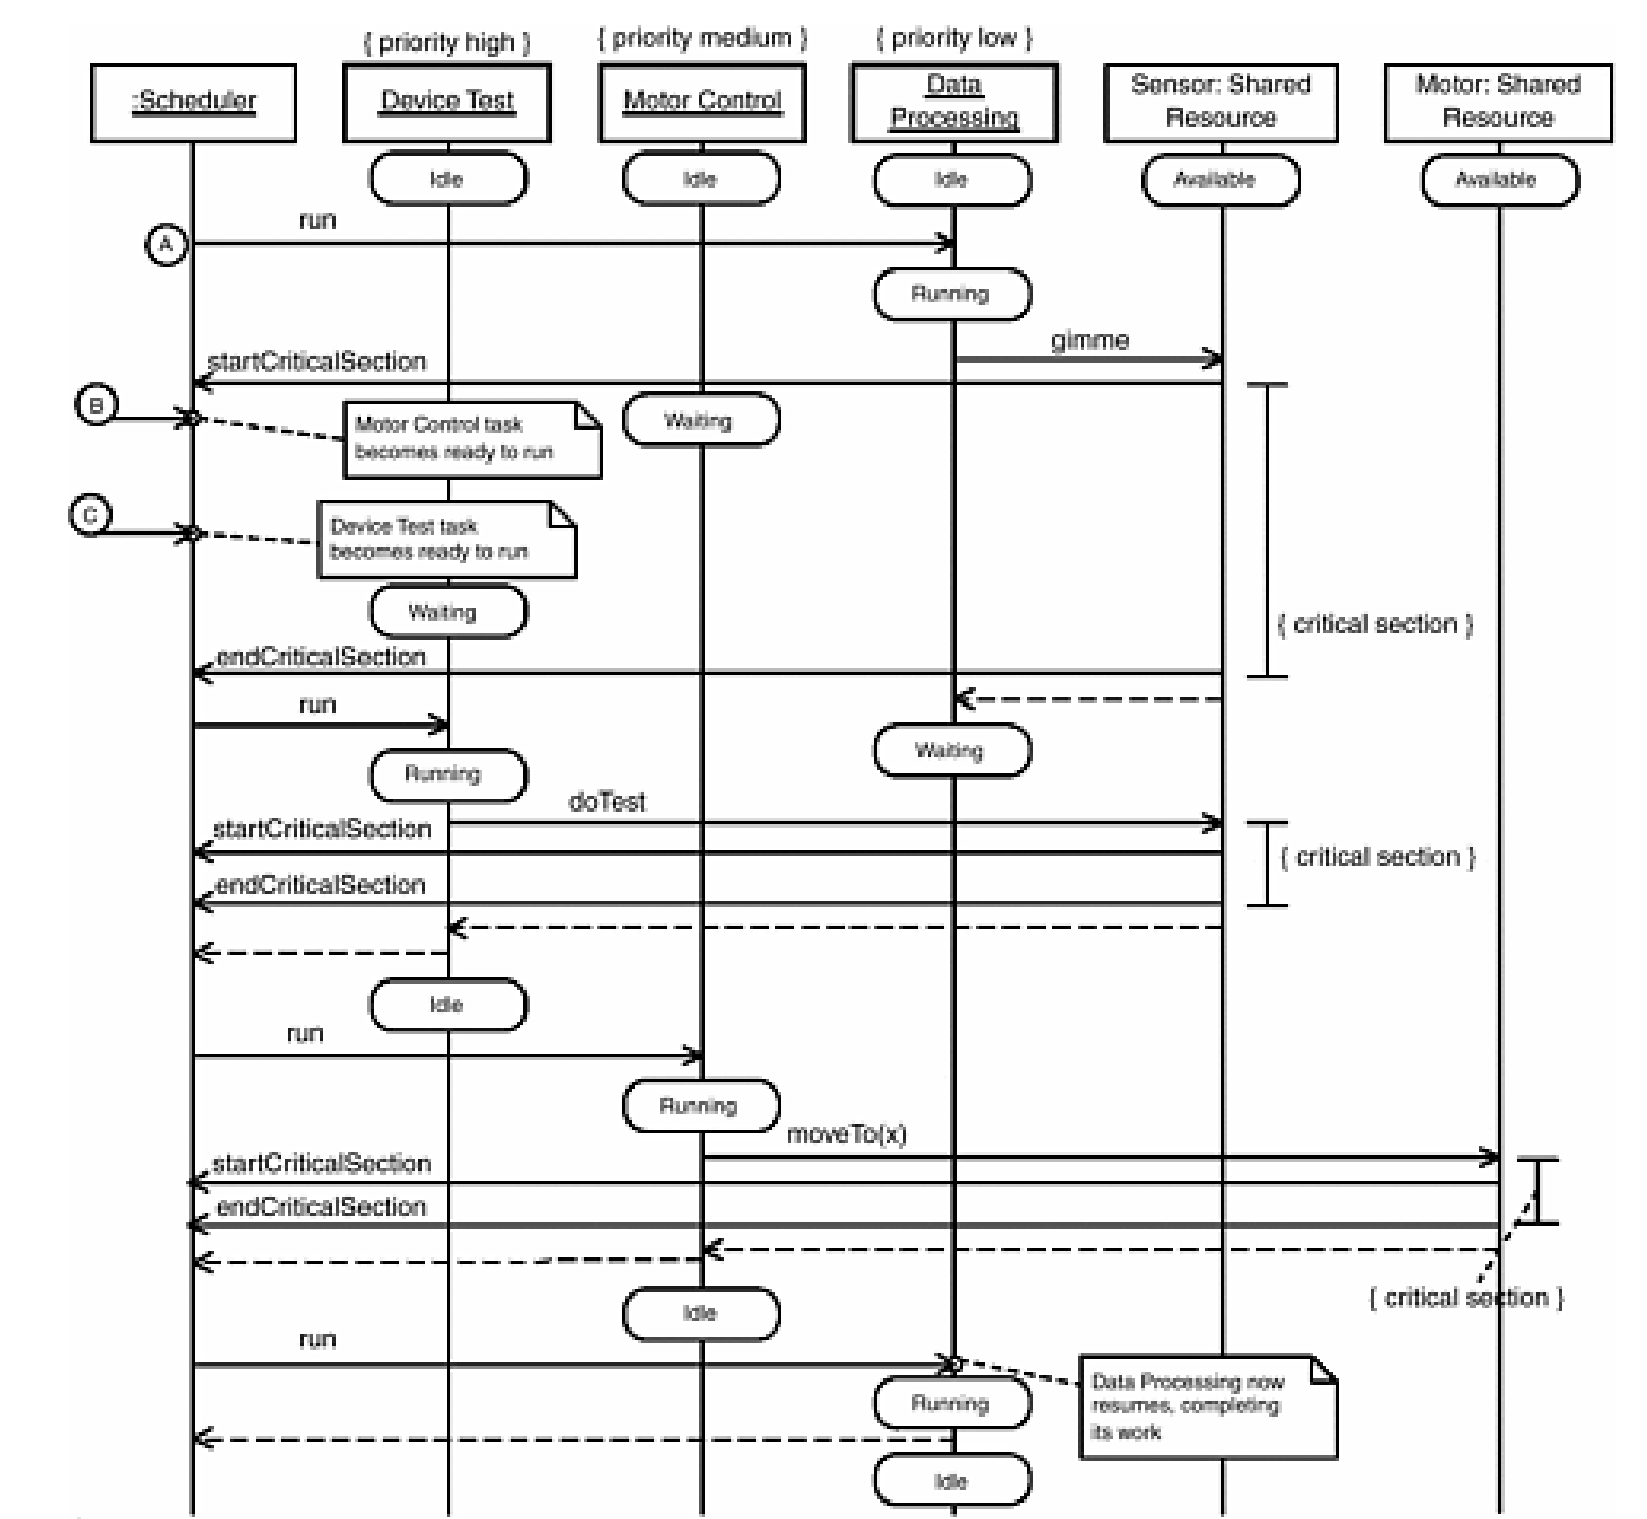
\includegraphics[width=0.5\textwidth]{npp_model}
    \caption{Sample Model for Non-Preemptive Protocol \cite{b6}}
    \label{fig:npp_model}
\end{figure}

\subsection{Problem Arise}

As shown in figure \ref{fig:Example_in_which_NPP_causes_unnecessary_blocking_on_T1}, this protocol will block highest priority task $ \tau_{1} $ even though the task will not access the resource.This problem could be solved in the next protocol which is Highest Locker Priority (HLP) protocol.

\begin{figure}[h]
    \centering
    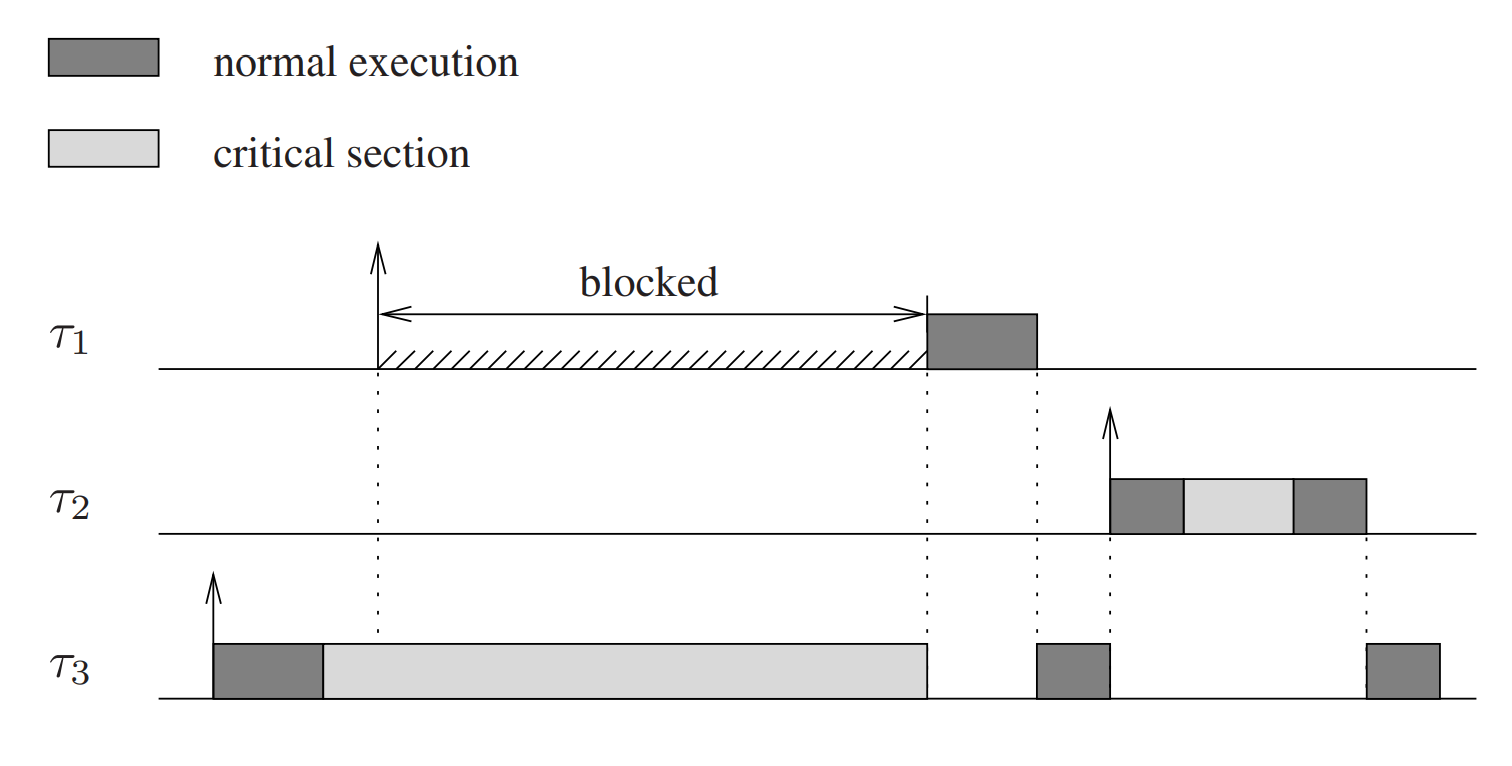
\includegraphics[width=0.5\textwidth]{Example_in_which_NPP_causes_unnecessary_blocking_on_T1}
    \caption{Example in which NPP causes unnecessary blocking on $ \tau_{1} $ \cite{b5}}
    \label{fig:Example_in_which_NPP_causes_unnecessary_blocking_on_T1}
\end{figure}



 
